\graphicspath{{sec02/images/}{sec02/code/}}
\lstset{inputpath=sec02/code/}


\begin{frame}[t]{Beamer}
    \begin{columns}
    \begin{column}{0.65\textwidth}
        \begin{block}{What is Beamer?}
            Beamer is a \LaTeX\ document class for creating slides for presentations. \\
            It supports pdflatex, latex+dvips, lualatex and xelatex.
        \end{block}
        \visible<2->{\url{https://ctan.org/pkg/beamer}}
    \end{column}
    \begin{column}{0.3\textwidth}
        \begin{center}
            
\includegraphics[width=.9\linewidth]{beamerlogo}
        \end{center}
    \end{column}
    \end{columns}
\end{frame}



\subsection{Document structure and style}
\graphicspath{{sec02/images/}{sec02/code/}}
\lstset{inputpath=sec02/code/}

\begin{frame}[fragile, label=simple]{Simplest Beamer document}\relax
    \cprotect\twocolImg{
        \inputminted{latex}{sec02/code/simplest01.tex}
    }{simplest01}
    \vspace{15mm}
    % \inclassFrag{Try it! \hyperlink{style}{\beamerbutton{STYLE}} }[-1]
    \skfootnote{\ccol{label=simple} at begin frame allows to get to the frame by \ccol\hyperlink command}
\end{frame}

\begin{frame}[fragile]{Beamer document structure}{like in regular document!}\relax
    \inputminted{latex}{sec02/code/structure.tex}
    
    \skfootnote{You can also use \ccol\frame\ command}
\end{frame}

\begin{frame}[fragile]{Title page (Preamble)}{like in regular document!}\relax
    \cprotect\twocolImg{
    \inputminted[firstline=5, lastline=17]{latex}{sec02/code/title.tex}
    % \lstinputlisting[linerange={5-17}]{title.tex}
    }{title}
\end{frame}



\begin{frame}[label=style,fragile]{Built--in themes}
    % \visible<1>{\hyperlink{simple}{\beamerbutton{SIMPLE}} \\}
    \lstinline[basicstyle=\tt]|\usetheme{CambridgeUS}|\\
    \lstinline[basicstyle=\tt]|\usecolortheme{crane}|\\
    \url{https://hartwork.org/beamer-theme-matrix/}\\ \pause
    \lstinline[basicstyle=\tt]|\usefonttheme{structureitalicserif}|\\
    \url{http://deic.uab.es/~iblanes/beamer_gallery/index_by_font.html}\\ 
    \vspace{1cm}
    \inclassFrag{Google \alert{Beamer Theme Matrix} and \alert{Beamer font theme gallery}.}[-1]
\end{frame}

\begin{frame}[fragile]{TOC ({\tt AtBeginSection[]})}\relax

    \begin{columns}
        \begin{column}{0.45\textwidth}
            \expandafter\inputminted[firstline=4, lastline=8]{latex}{sec02/code/toc.tex}
        \end{column}
        \begin{column}{0.45\textwidth}
            \includegraphics[width=\textwidth, keepaspectratio,page=6]{toc.pdf}
        \end{column}
    \end{columns}
    
\end{frame}


\begin{frame}[fragile]{Frame: Columns}\relax
    \cprotect\twocolImg{
    % \lstinputlisting[linerange={8-17}]{columns.tex}
    \inputminted[firstline=8, lastline=18]{latex}{sec02/code/columns.tex}
    }{columns.pdf}
    
    (\texttt{[t]} for ``top'' align)
\end{frame}


\begin{frame}[fragile]{Colors\preMagicPage}
    \skfootnote{\wikiC{https://en.wikibooks.org/wiki/LaTeX/Colors}}
    \LaTeX\ provides several standart colors: 
    \textcolor{red}{red}, \textcolor{blue}{blue}, \textcolor{green}{green},\dots\\
    \lstinline[basicstyle=\tt]|\textcolor{red}{text}| \\
    \pause
    There many ways to define new colors, e.~g.
    \lstinline[basicstyle=\tt]|\definecolor{orange}{rgb}{1,.5,0}|\\
    \lstinline[basicstyle=\tt]|\definecolor{orange}{RGB}{255,127,0}|
\end{frame}

\begin{frame}{Colors\magicPage}
    Beamer automatically loads \alert{xcolor} package\\
    Somehow popular way to define new colors is by the following rule
    \begin{table}
    \begin{tabular}{ccc}\hline
        color           &   rgb formula             &     output  \\\hline
        red!30!blue     &   .3(1,0,0)+.7(0,0,1)     &   \textcolor{red!30!blue}{example} \\
        red!30          &   .3(1,0,0)+.7(1,1,1)     &   \textcolor{red!30!}{example}    \\ 
        red!30!blue!50!green    &   .5(red!30!blue)+.5(0,1,0)   &   \textcolor{red!30!blue!50!green}{example}   
    \end{tabular}          
    \end{table}
\end{frame}

\begin{frame}[fragile]{Blocks \& Header customisation\magicPage}
        
    \cprotect\twocolImg{
    \inputminted[firstline=7, lastline=18]{latex}{sec02/code/custom.tex}
    }{custom}
        
\end{frame}


\begin{frame}[fragile]{Appendix\magicPage}\relax
    \begin{columns}
        \begin{column}{0.45\textwidth}
            \expandafter\inputminted[firstline=8, lastline=17]{latex}{sec02/code/appendix.tex}
        \end{column}
        \begin{column}{0.45\textwidth}
            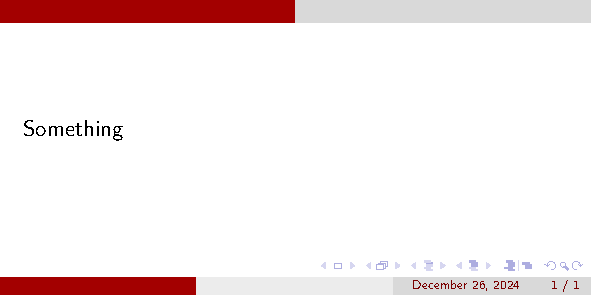
\includegraphics[width=\textwidth, keepaspectratio,page=1]{appendix}
            
            \includegraphics[width=\textwidth, keepaspectratio,page=2]{appendix}
        \end{column}
    \end{columns}
    
    (notice frame numbers!)
    
\end{frame}

\begin{frame}[fragile]{Bibliography (bibtex)\magicPage}\relax
    \cprotect\twocolImg{
    % \lstinputlisting[linerange={10-16}]{bibtex.tex}
    \inputminted[firstline=10, lastline=16]{latex}{sec02/code/bibtex.tex}
    }{bibtex.pdf}
\end{frame}

\begin{frame}[fragile]{Bibliography (simple)\magicPage}\relax
    \cprotect\twocolImg{
    % \lstinputlisting[linerange={9-21}]{bibliography.tex}
    \inputminted[firstline=9, lastline=21]{latex}{sec02/code/bibliography.tex}
    }{bibliography.pdf}
\end{frame}


\subsection{Tricks: overlays, animation, notes}
\graphicspath{{sec02/images/}{sec02/code/}}
\lstset{inputpath=sec02/code/}

\begin{frame}[fragile]{Stepwise viewing: \ccol\pause \preMagicPage}

    The \inpause main \inpause command \inpause to create \inpause pauses \inpause is \ccol\pause
\end{frame}

\begin{frame}[fragile]{Stepwise viewing\magicPage}
\skfootnote{\href{https://ctan.org/pkg/beamer}{man: sec 9.1}}
    Command \lstinline[basicstyle=\tt]|\pause|\pause\
    is the simplest way to create an overlay.
    \pause
    \[
        \zeta(s) = \sum^{\infty}_{k=1}{\frac{1}{k^s}},  \quad  \operatorname{Re}s > 1.
    \]
    \onslide\lstinline[basicstyle=\tt]|\onslide| command tells to show material from the first slide.\\
    \onslide+<3->\lstinline[basicstyle=\tt]|\onslide<3->| tells to show material from the third slide on.\\ 
    \pause \lstinline[basicstyle=\tt]|\pause| command then leads to the next slide.
\end{frame}

\begin{frame}[fragile]{Stepwise viewing\magicPage}
\skfootnote{\href{https://ctan.org/pkg/beamer}{man: sec 9}}
    Most of the commands are self--explanatory.\\
    \lstinline[basicstyle=\tt]|\pause<#>| --- following text shown only after slide \#  \\
    \lstinline[basicstyle=\tt]|\onslide<#>|  --- visible only slide \#\\
    \lstinline[basicstyle=\tt]|\FromSlide{#}| --- equivalent to \lstinline[basicstyle=\tt]|\onslide<#->|. \\
    \lstinline[basicstyle=\tt]|\only<#>| --- visible on particular slides, otherwise absent  \\
    \lstinline[basicstyle=\tt]|\uncover<#>| --- visible on particular slides, otherwise transparent \\
    \lstinline[basicstyle=\tt]|\visble<#>|  --- visible on particular slides, otherwise invisible  \\
    \lstinline[basicstyle=\tt]|\invisble<#>| --- opposite of \lstinline[basicstyle=\tt]|\visble<#>|. \\
    % \inclassFrag{Check the difference between \texttt{only} and \texttt{onslide} }[-1]
\end{frame}

\begin{frame}[fragile]{Overlays\magicPage}
    Overlay specifications can also be written together with some commands like 
    \lstinline[basicstyle=\tt]|\textbf|,
    \lstinline[basicstyle=\tt]|\item|,
    \lstinline[basicstyle=\tt]|\color|,
    \lstinline[basicstyle=\tt]|\alert|. \\
    \pause
    \lstinline[basicstyle=\tt]|\begin{enumerate}| \\
    \lstinline[basicstyle=\tt]|    \item<1-> Every \alert<3>{thing}|   \\
    \lstinline[basicstyle=\tt]|    \item<only@3,4> that has|   \\
    \lstinline[basicstyle=\tt]|    \item<2-> beginning| \\
    \lstinline[basicstyle=\tt]|    \item<1,4>  has end.|   \\
    \lstinline[basicstyle=\tt]|\end{enumerate}|
\end{frame}

\begin{frame}{Overlays\magicPage}
    \begin{enumerate}
        \item<1-> Every \alert<3>{thing}
        \item<only@3,4> that has
        \item<2-> beginning
        \item<1,4> has end.
    \end{enumerate}
\end{frame}

% \cprotect\inclassFrame{
% \begin{frame}[fragile]{Can you guess what does this code produce?}\relax
%     \lstinline[basicstyle=\tt]|\begin{itemize}[<+->]| \\
%     \lstinline[basicstyle=\tt]|    \item Every thing|   \\
%     \lstinline[basicstyle=\tt]|    \item that has|   \\
%     \lstinline[basicstyle=\tt]|    \item beginning| \\
%     \lstinline[basicstyle=\tt]|    \item has end.|   \\
%     \lstinline[basicstyle=\tt]|\end{itemize}|
% \end{frame}
% }

\begin{frame}{Overlays}
    \begin{itemize}[<+->]
        \item Every thing
        \item that has
        \item beginning
        \item has end.
    \end{itemize}
\end{frame}

\begin{frame}{Animation\magicPage}

    \transduration<1-4>{.5}
    \begin{itemize}
        \temporal<1>{\color{gray}}{\color{blue}}{\color{red!75}}{\item Every thing}
        \temporal<2>{\color{gray}}{\color{blue}}{\color{red!75}}{\item that has}
        \temporal<3>{\color{gray}}{\color{blue}}{\color{red!75}}{\item beginning}
        \temporal<4>{\color{gray}}{\color{blue}}{\color{red!75}}{\item has end.}
    \end{itemize}\vspace{5mm}
    \visible<5>{Cool, right?}
\end{frame}

\begin{frame}[fragile]{Animation\magicPage}
    \lstinline[basicstyle=\tt]|\animate<1-4>| \\
    \lstinline[basicstyle=\tt]|\begin{itemize}[<+->]| \\
    \lstinline[basicstyle=\tt]|    \item Every thing|   \\
    \lstinline[basicstyle=\tt]|    \item that has|   \\
    \lstinline[basicstyle=\tt]|    \item beginning| \\
    \lstinline[basicstyle=\tt]|    \item has end.|   \\
    \lstinline[basicstyle=\tt]|\end{itemize}|
\end{frame}

\begin{frame}[fragile]{Animation\magicPage}
    \lstinline[basicstyle=\tt]|\transduration<1-4>{.5}| \\
    \lstinline[basicstyle=\tt]|\begin{itemize}[<+->]| \\
    \lstinline[basicstyle=\tt]|    \item Every thing|   \\
    \lstinline[basicstyle=\tt]|    \item that has|   \\
    \lstinline[basicstyle=\tt]|    \item beginning| \\
    \lstinline[basicstyle=\tt]|    \item has end.|   \\
    \lstinline[basicstyle=\tt]|\end{itemize}|
\end{frame}

\inclassframe{
\begin{frame}{\exFrame{Create a presentation}}{lvl 1}\relax
     Create a beamer presentation with
     \begin{itemize}
         \item at least two slides
         \item title slide 
         \item at least two sections and table of content
     \end{itemize}
\end{frame}

\begin{frame}{\exFrame{Create a presentation}}{lvl 2}\relax
     Create a beamer presentation with
     \begin{itemize}
         \item at least two slides
         \item title slide 
         \item at least two sections and table of content
         \item at least two subsections
         \item with a slide at begin of every section and every subsection
         \item with any of the themes not uncovered above
         \item with overlayed list:
         \begin{itemize}
             \item firstly show only 1, 3, 5 item 
             \item secondly show only 1, 2 and 4 item
         \end{itemize}
     \end{itemize}
\end{frame}
}
